\documentclass[border=10pt]{standalone}
\usepackage{pgfplots}
\pgfplotsset{compat=1.17}
\begin{document}
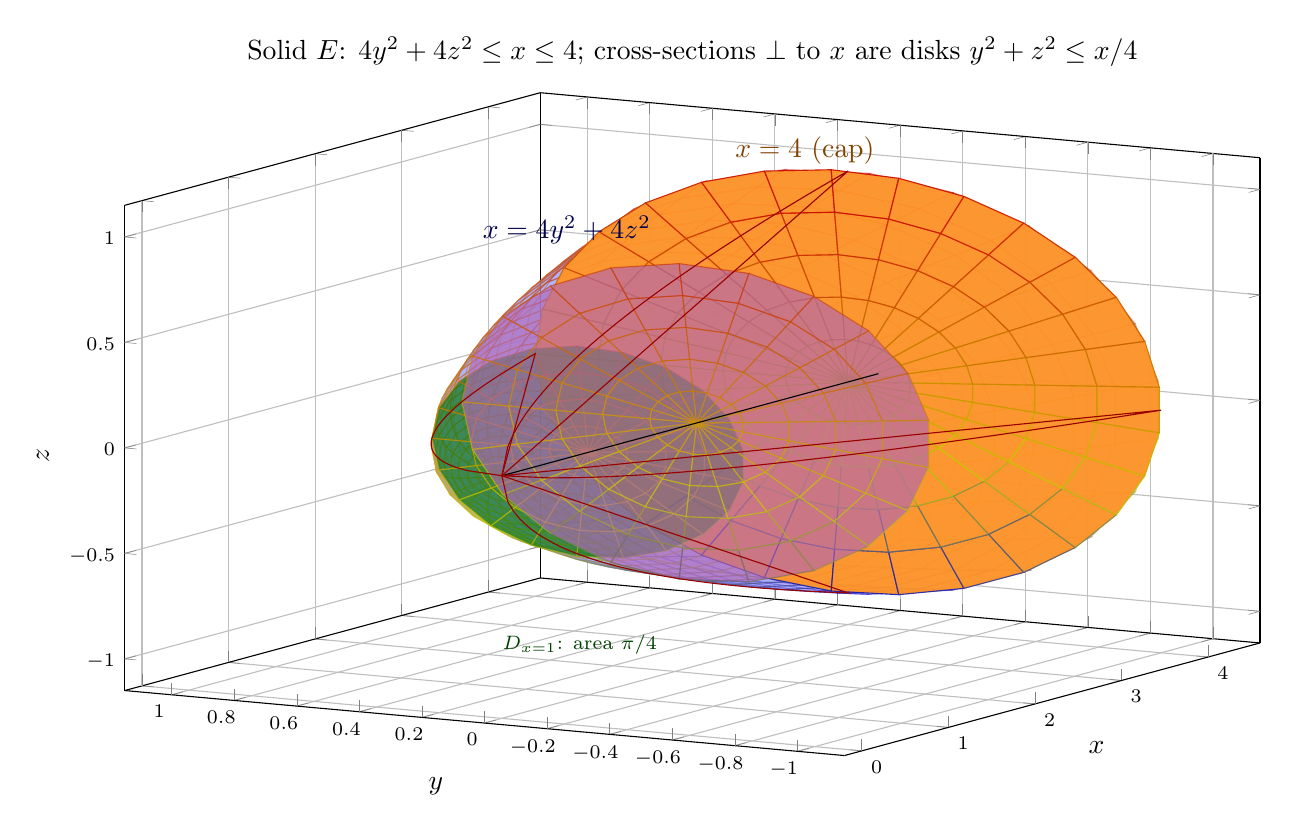
\begin{tikzpicture}
\begin{axis}[
    width=16cm, height=10cm,
    xlabel={$x$}, ylabel={$y$}, zlabel={$z$},
    xmin=-0.2, xmax=4.6, ymin=-1.15, ymax=1.15, zmin=-1.15, zmax=1.15,
    view={-60}{15},
    grid=major,
    title={Solid $E$: $4y^2+4z^2 \le x \le 4$;  cross-sections $\perp$ to $x$ are disks $y^2+z^2 \le x/4$},
    tick label style={font=\scriptsize},
]
% paraboloid x = 4(y^2+z^2)
\addplot3[surf, shader=faceted, color=blue!40, opacity=0.5,
          domain=0:1, y domain=0:360, samples=24, samples y=24, z buffer=sort]
    ({4*x^2}, {x*cos(y)}, {x*sin(y)});
% cap disk x = 4
\addplot3[surf, shader=faceted, color=orange!85, opacity=0.95,
          domain=0:1, y domain=0:360, samples=6, samples y=30, z buffer=sort]
    (4, {x*cos(y)}, {x*sin(y)});
% cross-section disk D_{x=1}: radius 0.5
\addplot3[surf, shader=faceted, color=green!45!black, opacity=0.65,
          domain=0:0.5, y domain=0:360, samples=5, samples y=22, z buffer=sort]
    (1, {x*cos(y)}, {x*sin(y)});
% cross-section disk D_{x=2.25}: radius 0.75
\addplot3[surf, shader=faceted, color=violet!60, opacity=0.65,
          domain=0:0.75, y domain=0:360, samples=6, samples y=22, z buffer=sort]
    (2.25, {x*cos(y)}, {x*sin(y)});
% axis of symmetry
\addplot3[black, dashed, thin, domain=0:4.35, samples=2] (x, 0, 0);
% silhouette parabolas (on the surface), thin
\addplot3[red!60!black, thin, domain=0:4, samples=60] (x, {sqrt(x)/2}, 0);
\addplot3[red!60!black, thin, domain=0:4, samples=60] (x, {-sqrt(x)/2}, 0);
\addplot3[red!60!black, thin, domain=0:4, samples=60] (x, 0, {sqrt(x)/2});
\addplot3[red!60!black, thin, domain=0:4, samples=60] (x, 0, {-sqrt(x)/2});
% labels
\node[color=blue!30!black] at (axis cs:0.75,0,1.08) {$x=4y^2+4z^2$};
\node[color=orange!50!black] at (axis cs:3.5,0,1.15) {$x=4$ (cap)};
\node[color=green!25!black] at (axis cs:0.9,0,-0.9) {\scriptsize $D_{x=1}$: area $\pi/4$};
\end{axis}
\end{tikzpicture}
\end{document}